
\begin{task}{4, Obstacle avoidance}
The starting point was to create a heap with decrease key data structure. The decrease function was implemented through integer IDs. After every add an ID was returned (simply the number of times add was called on the particular heap beforehand), this seams like a cleaner implementation than using the python id method or some hashing function as it is language oblivious, doesn't necessitate keeping the original object around and allows for the same values to occur multiple times with different keys if necessary. The first implementation was a simple list heap with O(N) time complexity. This was later changed into a binary tree in list heap.

The Dijkstra's algorithm implementation was originally a path finding one because the author had miss-read the problem definition. The author was of the belief that it was necessary to calculate the distance from each position to the targets by starting the Dijkstra's algorithm at the position while it is of course elementary to instead start at the target and work one's way backward. In hopes of somehow decreasing the substantial runtime this caused the author tried to make the Heap more efficient by using numpy arrays instead of lists of tuples. Turning the algorithm into an A* by adding a euclidian distance heuristic was also tried. In the end it turned out this was not enough and the author soon discovered his error and that these additions were not necessary, so they were removed from the final code. The implementation was made modular by making the distance and neighborhood functions it's parameters of type typing.Callable.

For implementing the Fast Marching Method algorithm all that was necessary was to realize that having implemented Dijkstra's algorithm all that was required to implement the Fast Marching Method was to add a dictionary with distances to closed keys as a parameter to the distance function. All that was needed then was to pass a Fast Marching Method distance update function as a distance function to the Dijkstra's algorithm implementation.

The Fast Marching Method distance update is based on the simple idea that if the derivative of the distance between neighboring nodes is to be constant the identity
$$max(D_{0,0}-D_{1,0}, D_{0,0}-D_{-1,0})^2 + max(D_{0,0}-D_{0,1}, D_{0,0}-D_{0,-1})^2 - C = 0  $$
must hold. Where $D_{0,0}$ is the distance to the updated node at position a,b and $D_{x,y}$ is simply the node at position (a+x,b+y). C being the square of the derivative of the distance function which in our case where we use the Fast Marching Method only for distance calculation is an arbitrary positive number, though 1 seems to work the best as at larger numbers the method's inaccuracy increases.
All we need to get the update is to get the greater of the roots of this polynomial.
In case there is no such root we simply use the approximate expression
$$\frac{-b}{2a}$$
where b is the first power multiplier in the polynomial and a the second power one.

In cases where there is another value in the direction of the maximum distance we can use the second order Fast Marching Method, this has been implemented in the project but describing the theory behind it seems out of scope of this work.

The user interface function \verb+path_lengths+ was for the user's ease of use made to only take a neighborhood function and \verb+is_obstacle+ function, with a simple enum used to choose between different implementations.

As stated before using this implementation in the application was as simple as calling the function for every target with the neighborhood function set to either adjacent for the Fast Marching Method implementation or adjacent+diagonal for the Dijkstra's algorithm implementation, the obstacle function simply checking whether the grid contains and obstacle at given position and recording the minimum resultant distance for each cell.

\paragraph{Pedestrian avoidance}
As instructed we only take into consideration obstacles and ignore pedestrians while calculating distances. This significantly reduces computational complexity but forces any pedestrian avoidance to have a purely greedy character. Of course in most ways this is exactly the behaviour that makes most sense as humans are generaly very poor at predicting the behaviour of other humans in a crowd over any longer period of time. We implement this through a simple cost function. To calculate this for cost for a target position the algorithm takes the count of pedestrians at a given surrounding position and multiplies them with weights we assign based on the offset from the target position. These weights are a dictionary of weights decreasing exponentially with euclidian distance of the key from the center of the matrix.

$$
f(d) =
     \begin{cases}
       exp(\frac{p}{d^2-d_{max}^2}) \ \text{if $d < d_{max}$}\\
       0 \ \text{otherwise}\\
     \end{cases}
$$

$p$ being the parameter determining how fast $f$ decreases.

To allow for easier manipulation these values are then normalized.

Setting $p$ too low can cause clustering into lines or points since the small distance positions occur less frequently than the high distance ones. It would therefore seem reasonable that at least half the distribution be at the position (0,0).

In general because the complexity of the calculation increases with the square of $d_{max}$ with the python implementation values greater than 10 decrease the speed of the simulation. Then again multipliers of less than 0.01 (which such a distribution would have even were it uniform) hardly contribute much. These are especially preelent if we want at least half the distribution be near the center. Therefore if we explicitly ignore such small multipliers most reasonable distributions of any size are computationally reasonable for given pedestrian counts. This needs pre-computing the values and caching them instead of calculating the coefficient during every cost calculation as it was originally, this doesn't have much impact on the complexity neither positive or negative (apart from the aforementioned ability to ignore small coefficients). It also allows for the code to be more modular as we can theoretically pass any coefficient dictionary to the function.

\paragraph{Experiment description}
In this experiment we perform the RiMEA-12 test according to \cite{rimea2016}, where pedestrians have to pass a tight hallway. This experiment should show that pedestrians will form a congestion only at the first bottleneck. Notably here are the different CLI prompts we can use to simulate different pedestrian avoidance behaviour. By default we run the following command:
\begin{verbatim}
python main.py --scenario scenario-RIMEA-12.json
\end{verbatim}
Use the flag \verb+--multiplePedestriansInOneCell+ to change the behaviour of pedestrian avoidance. If the flag \verb+--ignorePedestrians+ is set before pedestrian avoidance will be completely disabled, hence setting the flag \verb+--multiplePedestriansInOneCell+ does nothing. 

If the simulation with no flags is run we observe the following figures \ref{rimea12}a, \ref{rimea12}b and \ref{rimea12}c to show the behaviour in the bottleneck scenario. When presented with the bottleneck the pedestrians are forced to wait as the cost of being forced through the bottleneck all at once is too high. The pedestrians also immediately disperse again after leaving the bottleneck to minimize their cost.

\begin{figure}[H] 
\centering
\subfigure[Congested pedestrians]{
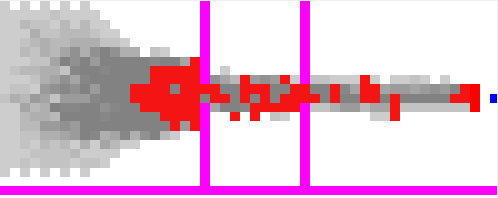
\includegraphics[scale=0.4]{image/Bottleneck-start}}
\subfigure[Pedestrians flowing through after bottleneck ended]{
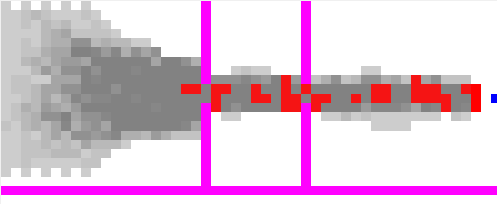
\includegraphics[scale=0.4]{image/Bottleneck-trickle}}
\subfigure[Bottleneck end]{
 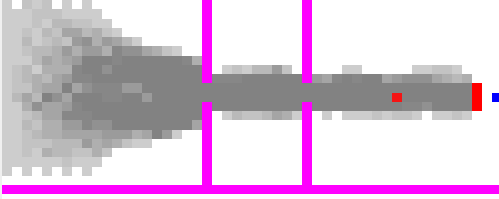
\includegraphics[scale=0.4]{image/Bottleneck-end}}
\subfigure[Bottleneck speeds]{
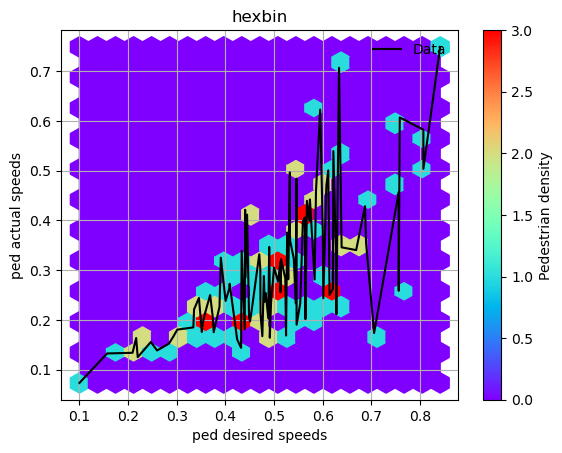
\includegraphics[scale=0.45]{report-template/image/bottleneck-speeds.png}}
\caption{RiMEA-12 simulation}
\label{rimea12}
\end{figure}

It seems that the blockage causes the actual speeds to not correlate as much with the desired speeds. We can observe this better if we don't use pedestrian avoidance in the same scenario. In Figure \ref{rimea12withoutped}a and \ref{rimea12withoutped}b we can see that now there is no bottleneck and pedestrians follows a straightforward path to the target, with no need for waiting the other pedestrians. This saved time is exhibited in Figure \ref{rimea12withoutped}c, where the speeds are more uniformly and linearly distributed, showing that pedestrians have made the way according to their desired speed, instead of reducing the actual speed due to the bottleneck. Also, analyzing the graph, we can observe that, naturally, without bottleneck there is more density of pedestrians with equivalent desired\_speed/actual\_speed ratio, as pedestrians can move freely. The maximum density in Figure \ref{rimea12}d is 3 and in \ref{rimea12withoutped}c is 6.
\begin{figure}[H] 
\centering
\subfigure[No bottleneck]{
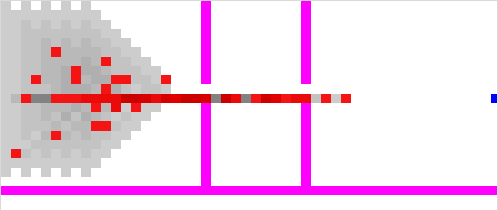
\includegraphics[scale=0.4]{report-template/image/rimea12withoutped.png}}
\subfigure[More advanced step in simulation]{
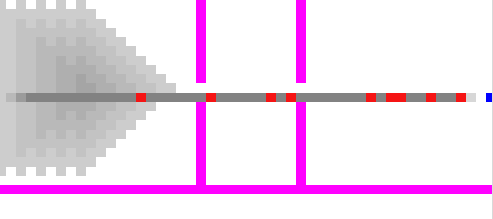
\includegraphics[scale=0.4]{report-template/image/finalwithoutped.png}}
\subfigure[No bottleneck speeds]{
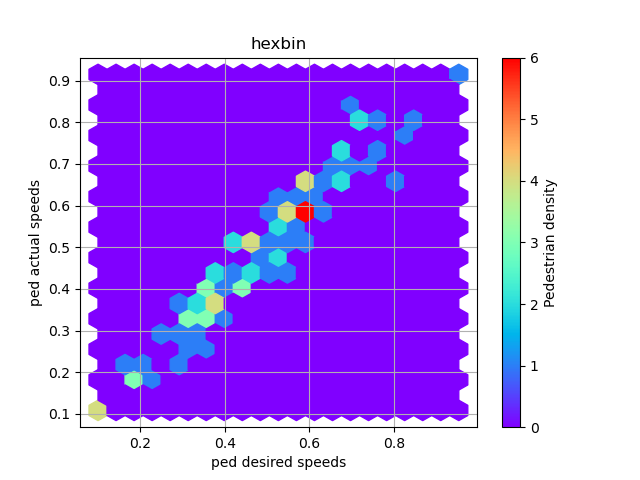
\includegraphics[scale=0.45]{report-template/image/rimea12graphnoped.png}}
\caption{RiMEA-12 simulation without pedestrian avoidance}
\label{rimea12withoutped}
\end{figure}

Then, in the chicken test if we simply use distance to target as path to target cost, thus ignoring obstacles, the pedestrian gets stuck at the first intersection of a line to the target and the obstacle (Figure \ref{chickentest}a). However, if we calculate the distance to the target using Fast Marching, the pedestrian can find an optimal path (Figure \ref{chickentest}c). Going deeper, by changing the background to the computed distances by the algorithm in use, we can analyse the cause of the problem, as it can be seen in Figure \ref{chickentest}b and \ref{chickentest}d. The pedestrian has a more informed distance measurement using the Fast Marching Method. The CLI prompts for \ref{chickentest}a and and \ref{chickentest}c are respectively:
\begin{verbatim}
python main.py --scenario chicken_test.json --algorithm S

python main.py --scenario chicken_test.json --algorithm F 
\end{verbatim}


\begin{figure}[H] 
\centering
\subfigure[Chicken test no path finding]{
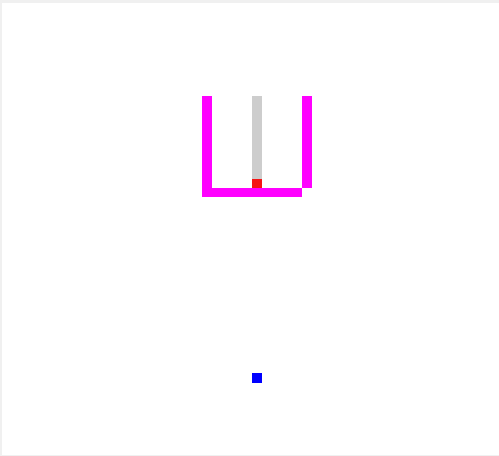
\includegraphics[width=0.35\textwidth]{report-template/image/chicken-test-dumb.png}}
\subfigure[Standard algorithm visual test]{
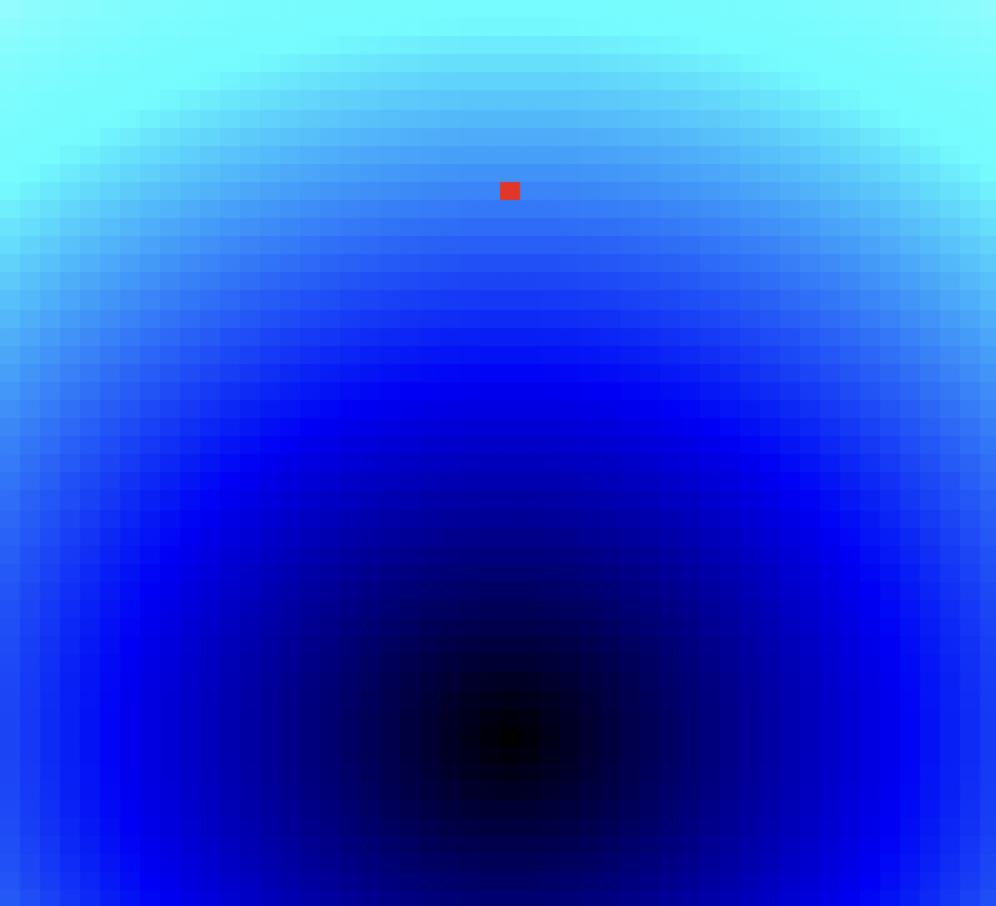
\includegraphics[width=0.35\textwidth]{report-template/image/chicken_dumb_vis.png}}
\subfigure[Chicken test with path finding]{
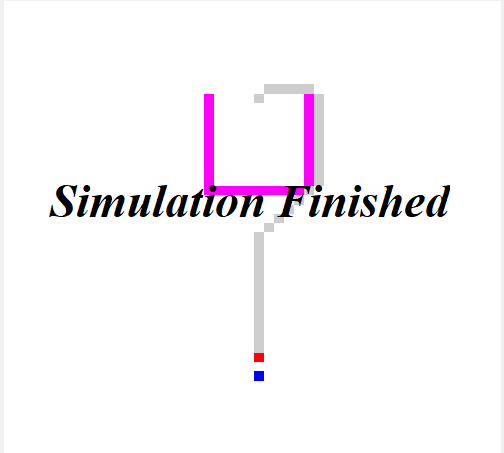
\includegraphics[width=0.35\textwidth]{report-template/image/chicken-test-clever.png}}
\subfigure[FMM visual test]{
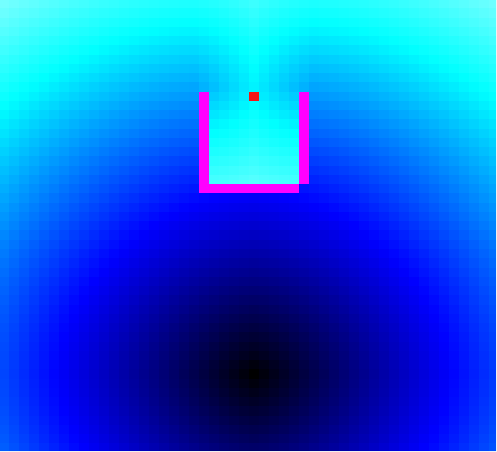
\includegraphics[width=0.35\textwidth]{report-template/image/fmm-visual-test.png}}
\caption{Chicken test simulation}
\label{chickentest}
\end{figure}


\end{task}



